\documentclass[aspectratio=43,scheme=plain]{ctexbeamer}
%\usepackage{xeCJK}
\setCJKmainfont{IPAexGothic}

%\usetheme{Antibes}
%\setbeamertemplate{navigation symbols}{\thepage}
%\setbeamertemplate{caption}[numbered]
%\usecolortheme{dove}

\usetheme{trigon}
\trigonset{titlestyle=style2,
	sectionpage=none,
	headingcolor=theme,
	numbering=fraction,
	block=fill
}
\setcounter{tocdepth}{2}
%\usetheme[nofirafonts,numbering=progressbar,totalframenumbering=yes]{focus}

%\usetheme[showmaxslides,customfont,nofooter]{pureminimalistic}
%\renewcommand{\logotitle}{}
%\renewcommand{\logoheader}{}
%\renewcommand{\logofooter}{}

%\usetheme[numbering=fraction,progressbar=frametitle,sectionpage=none,block=fill,subsectionpage=none]{metropolis}

\usepackage{pgfpages}
%\pgfpagesuselayout{4 on 1}[a4paper,landscape]
%\setbeameroption{show notes on second screen=right}
\AtBeginSection[]{
	\begin{frame}{Contents}
		\tableofcontents[currentsection]
\end{frame}}

\AtBeginSubsection[]{
	\begin{frame}{Contents}
		\tableofcontents[currentsection,currentsubsection]
\end{frame}}
\usefonttheme{professionalfonts}

\usepackage{siunitx}
\usepackage[version=4]{mhchem}
\usepackage{amsmath}
\usepackage{amssymb}
\usepackage{amsfonts}
\usepackage{metalogo}
\usepackage{appendix}
\usepackage{xcolor}
%\pagecolor[RGB]{46,46,46}
%\color[RGB]{248,248,248}
\usepackage{framed}
\usepackage{tabularx}
\usepackage{colortbl}
\usepackage{enumerate}
\usepackage{wrapfig2}
\usepackage{graphicx}
\usepackage{subfigure} 
\usepackage{float} 
\usepackage{tikz}
\usepackage{qrcode}
\usepackage{booktabs}
\usepackage{multirow}

\renewcommand{\appendixtocname}{付録}
\renewcommand{\appendixpagename}{付録}
\renewcommand{\contentsname}{目次}
\renewcommand{\figurename}{Fig.}

\usepackage[hyperref=true,backend=biber,url=false,doi=false,dateabbrev=true,backref=false,maxnames=2]{biblatex}
\DeclareFieldFormat{biblabeldate}{\mkbibparens{\mkbibbold{#1}}}
\DeclareFieldFormat[article,periodical]{volume}{\mkbibbold{#1}}
\renewbibmacro{in:}{}
\addbibresource{reference.bib}%导入bib文件。

%\usepackage{hyperref}
\hypersetup{
	bookmarksnumbered=true,
	colorlinks=false,
	linkcolor=black,
	urlcolor=black,
	citecolor=black,
	pdfauthor={B4},
	pdfcreator={XYX},
	pdftitle={Machine time report},
	pdfsubject={Galvano, },
	pdfkeywords={Exercise experiments}
}

\title{練習実験報告}
\author{肖宇笑}
\date{\today}
\begin{document}
%	\maketitle 						   %for Metropolis, Antibes, focus
	\titleframe						    %for Trigon
	\begin{frame}{Contents}
	\tableofcontents
	\end{frame}
	\section{Glavano Sepctrum}	
	\begin{frame}{\insertsection}
		\begin{figure}[H]
			\centering
			\begin{tikzpicture}
					\onslide<1>{\node at (0,0){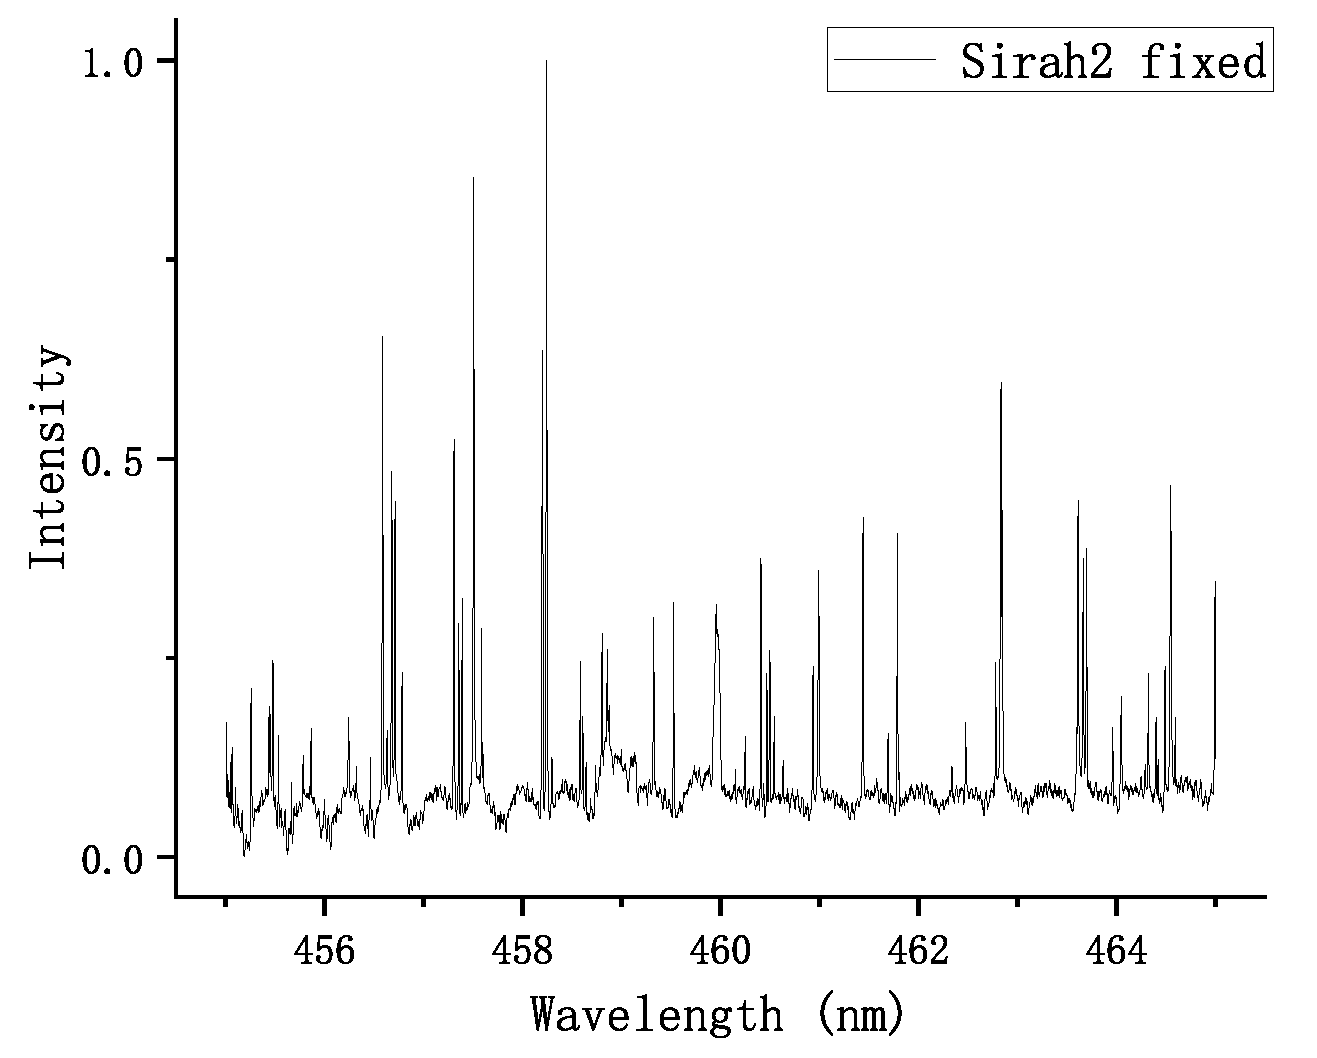
\includegraphics[width=0.6\textwidth]{sirah2fixed.eps}};}
					\onslide<2>{\node at (0,0){\includegraphics[width=0.6\textwidth]{wavelen_corrected.pdf}};}
			\end{tikzpicture}
			\caption{Wavelen. correction}
		\end{figure}
	\end{frame}
	\begin{frame}{\insertsection}{Correction}
		\begin{figure}[H]
			\centering
			\includegraphics[width=0.6\textwidth]{fitfunc.pdf}
			\caption{Correction function}
		\end{figure}
	\end{frame}
\section{REMPI scan}
\subsection{Selected peaks}
\begin{frame}{\insertsubsection}
\begin{figure}[H]
\centering
\begin{tikzpicture}
			\draw[white] (4.03,-3.65) rectangle (4,3.65);
			\node at (0,0){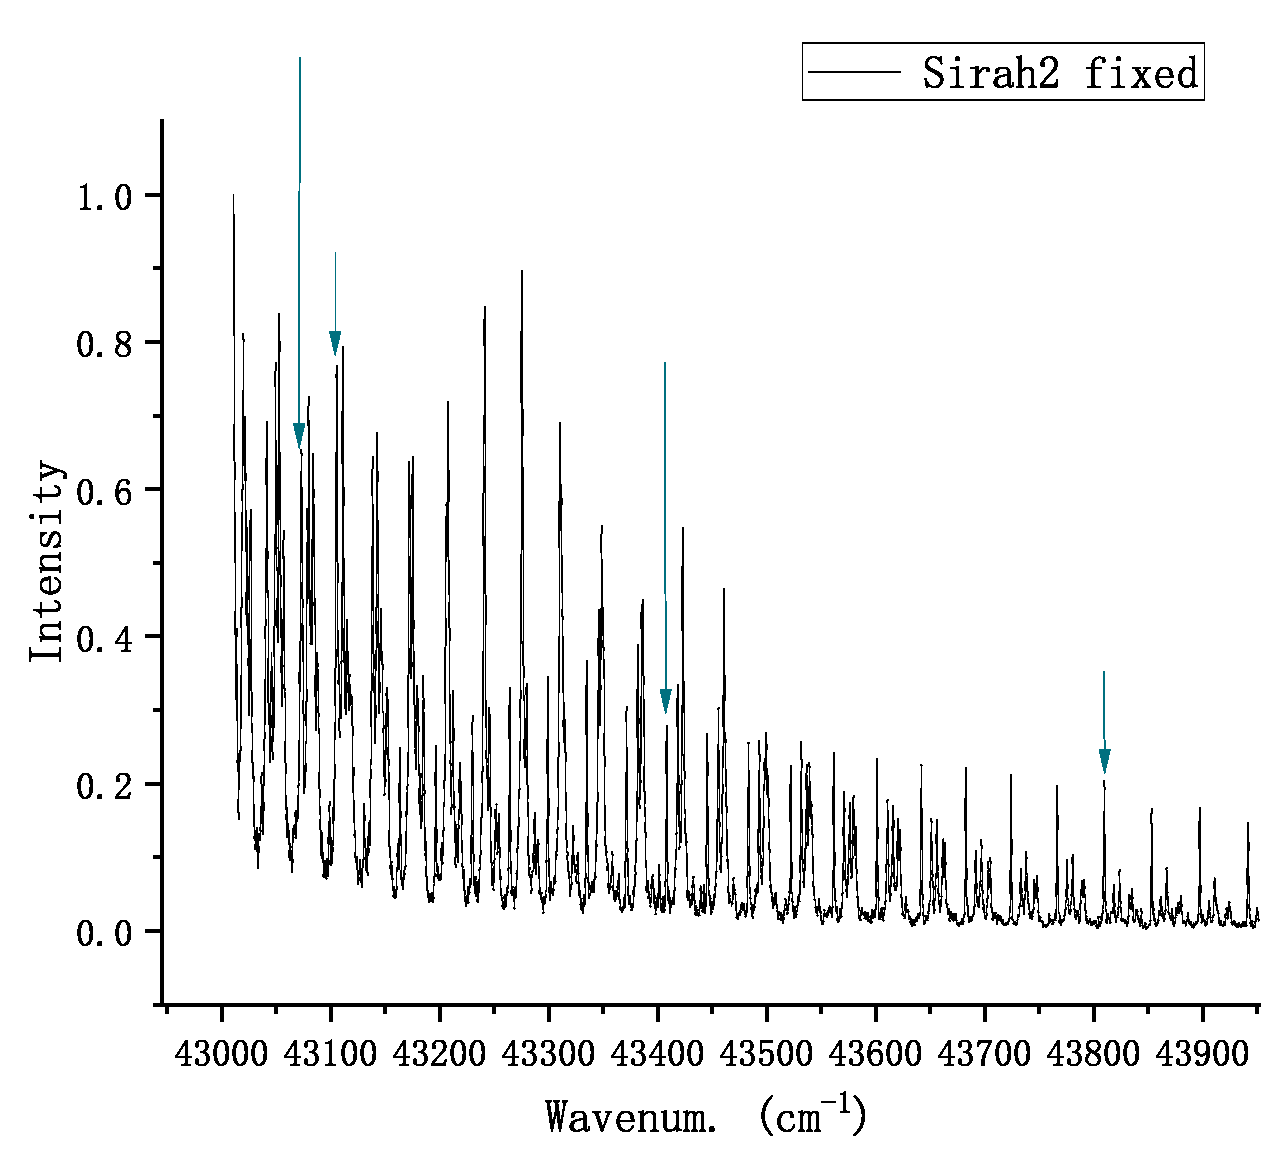
\includegraphics[width=0.6\textwidth]{scanmark.eps}};
			\filldraw[white] (-1.92,2.5) rectangle (-1.88,2.89);
			\node at (-1.5,2.7){\textcolor[RGB]{0,112,127}{$\num{464.484}\unit{\nano \meter}$}};
			\node at (-0.93,2.03){\textcolor[RGB]{0,112,127}{$\num{464.114}\unit{\nano \meter}$}};
			\node at (0.47,1.5){\textcolor[RGB]{0,112,127}{$\num{460.875}\unit{\nano \meter}$}};
			\node at (2.3,-0.25){\textcolor[RGB]{0,112,127}{$\num{456.659}\unit{\nano \meter}$}};
\end{tikzpicture}
\end{figure}
\end{frame}
\begin{frame}{Contents}
\tableofcontents[currentsection,currentsubsection]
\end{frame}
\subsection{Radius and angular distributions}
\begin{frame}{Peak 1}
	\begin{figure}[H]
		\centering
		\begin{tikzpicture}
	\onslide<1,2>{\node at (0,0){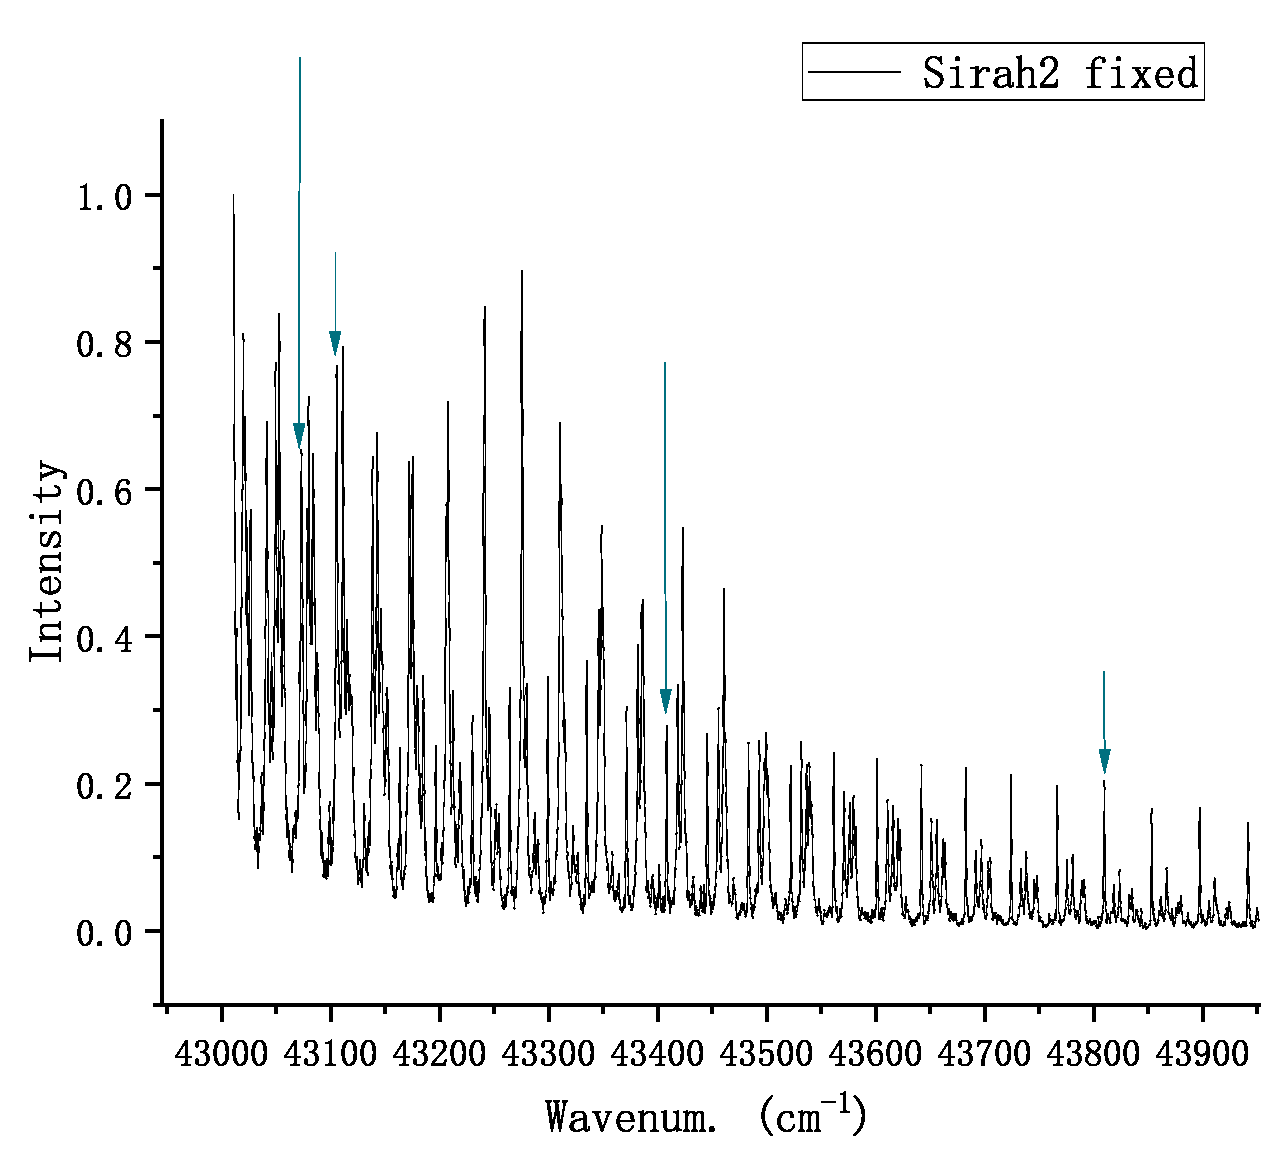
\includegraphics[width=0.6\textwidth]{scanmark.eps}};
	\filldraw[white] (-1.92,2.5) rectangle (-1.88,2.89);
	\node at (-1.5,2.7){\textcolor[RGB]{0,112,127}{$\num{464.484}\unit{\nano \meter}$}};
}
\onslide<2>{
	\node at (2.03,2.4){{\quad\!}rR2(44.5)};
	\node at (2.03,2){\textcolor{red}{{\quad\!}qR12(51.5)}};
	\node at (2.03,1.6){\textcolor{red}{{\quad\!}qQ2(51.5)}};
}
	\onslide<3>{\node at (-1.55,2){\includegraphics[width = 4cm]{gring_464355.eps}};
	\node at (2.45,2){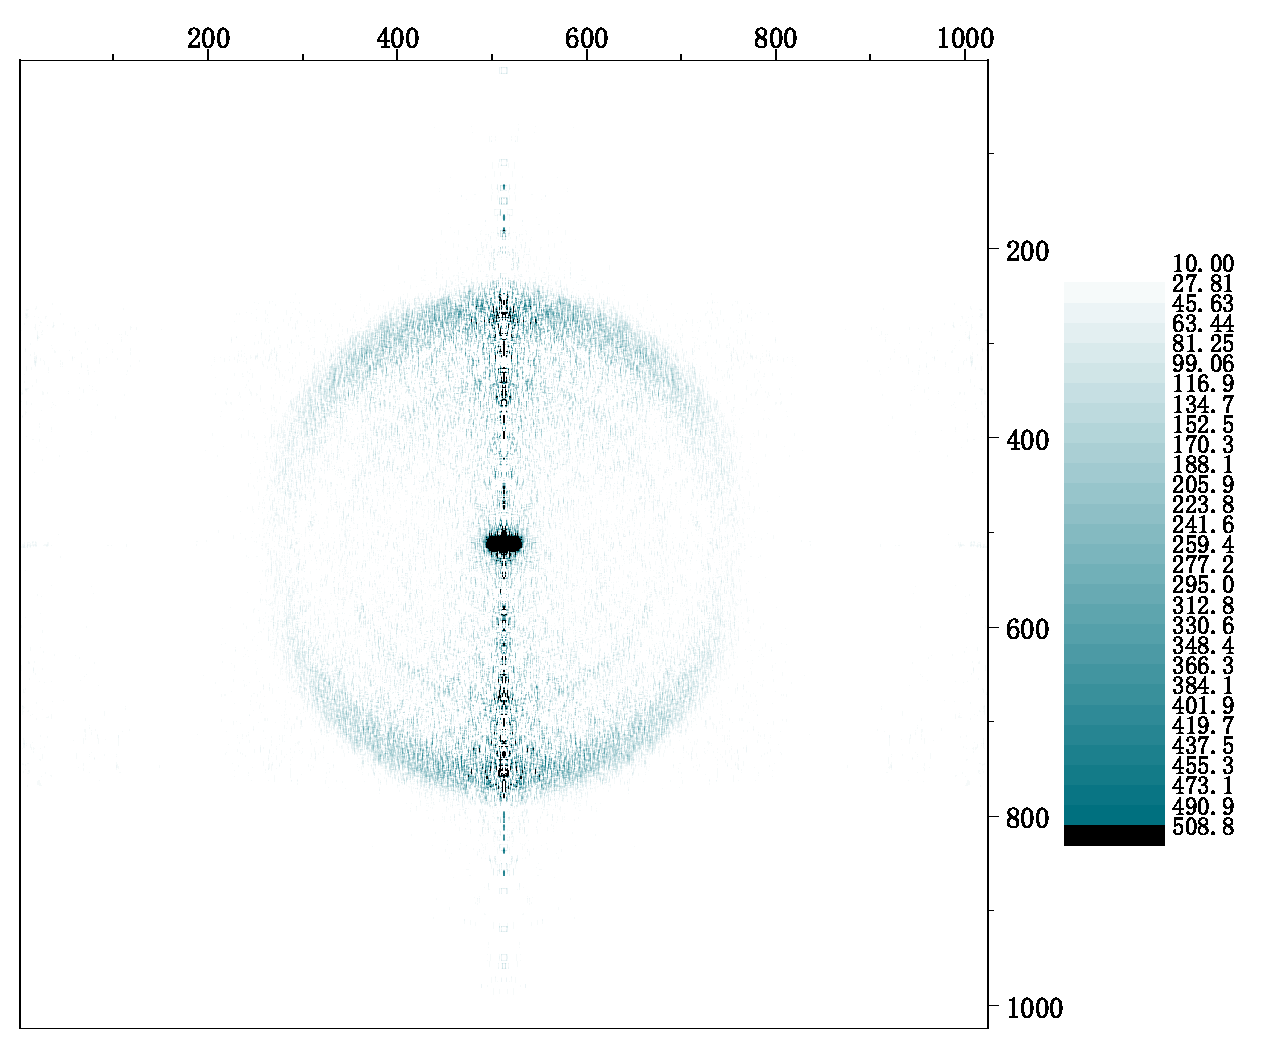
\includegraphics[width=4cm]{aring_464355.eps}};
	\node at (-2,-2){\includegraphics[width=4cm]{rdis_peak_464355.eps}};
	\node at (2,-2){\includegraphics[width=4cm]{adis_464355b.eps}};
	\node at (1.3,-3.2){\textcolor[RGB]{0,112,127}{\small $\beta \approx 1.52$}};
		\node at (-3.0,3.3){\textcolor[RGB]{0,112,127}{smear}};
	\node at (3.07,3.3){\textcolor[RGB]{0,112,127}{Abel${}^{-1}$}};}
\end{tikzpicture}
\end{figure}
\end{frame}
\begin{frame}{Peak 2}
	\begin{figure}[H]
		\centering
		\begin{tikzpicture}
	\onslide<1,2>{\node at (0,0){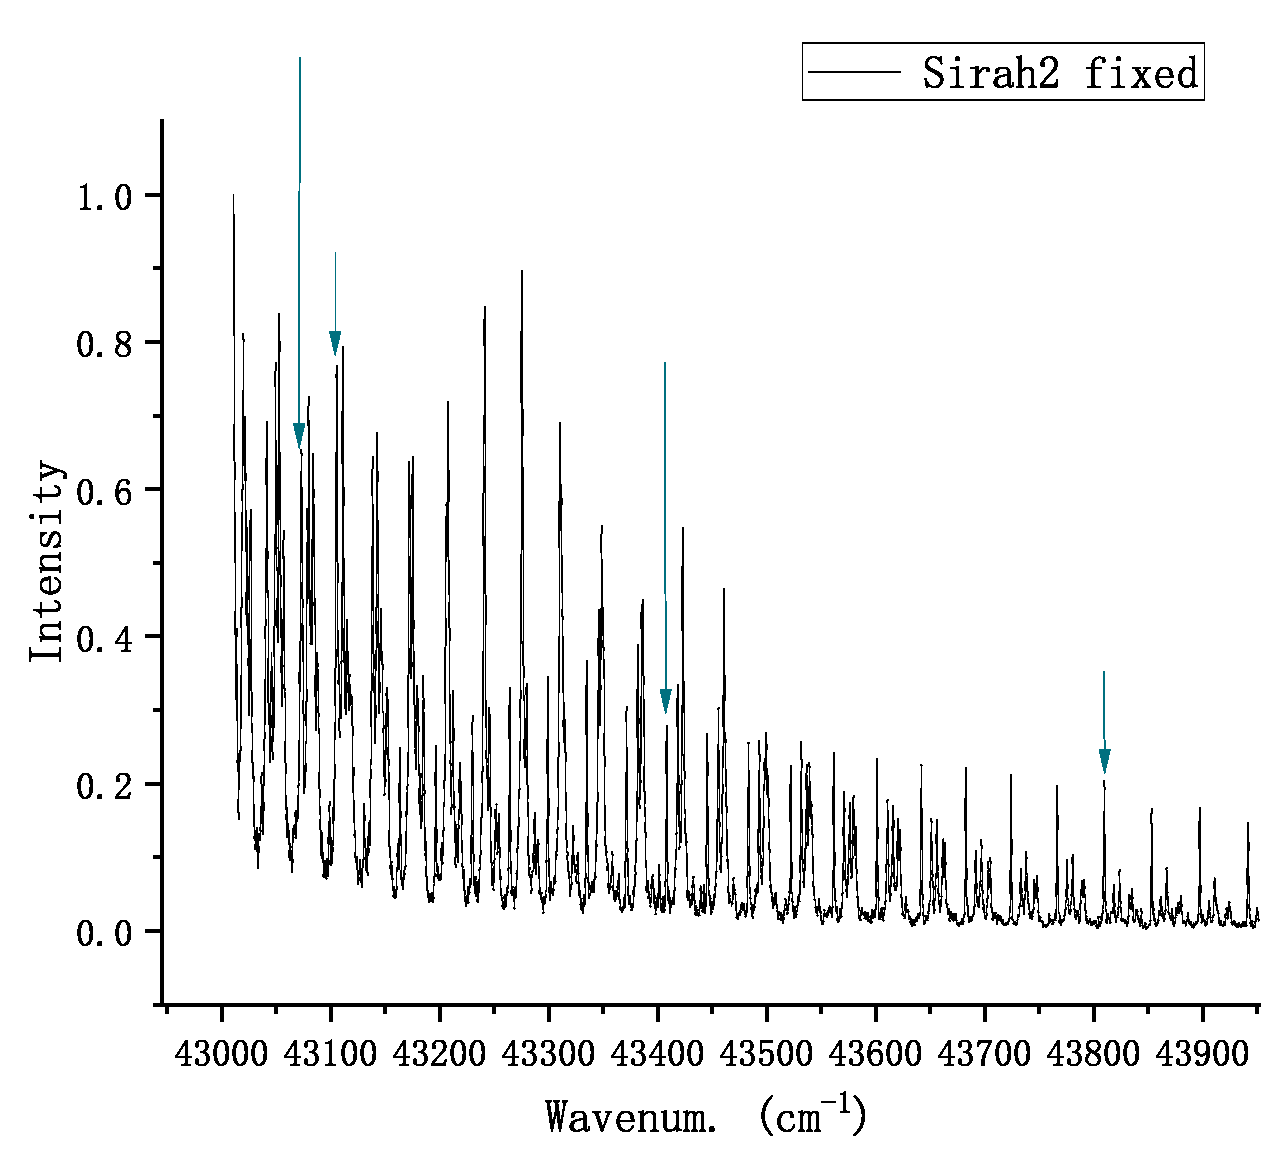
\includegraphics[width=0.6\textwidth]{scanmark.eps}};
	\filldraw[white] (-1.92,2.5) rectangle (-1.88,2.89);
			\node at (-0.93,2.03){\textcolor[RGB]{0,112,127}{$\num{464.114}\unit{\nano \meter}$}};
}
\onslide<2>{	
	\node at (2.03,2.4){{\quad\!}rR2(45.5)};
	\node at (2.03,2){\textcolor{red}{{\quad\!}qR12(51.5)}};
	\node at (2.03,1.6){\textcolor{red}{{\quad\!}qQ2(51.5)}};
}
		\onslide<3>{\node at (-1.55,2){\includegraphics[width = 4cm]{gring_463985.eps}};
			\node at (2.45,2){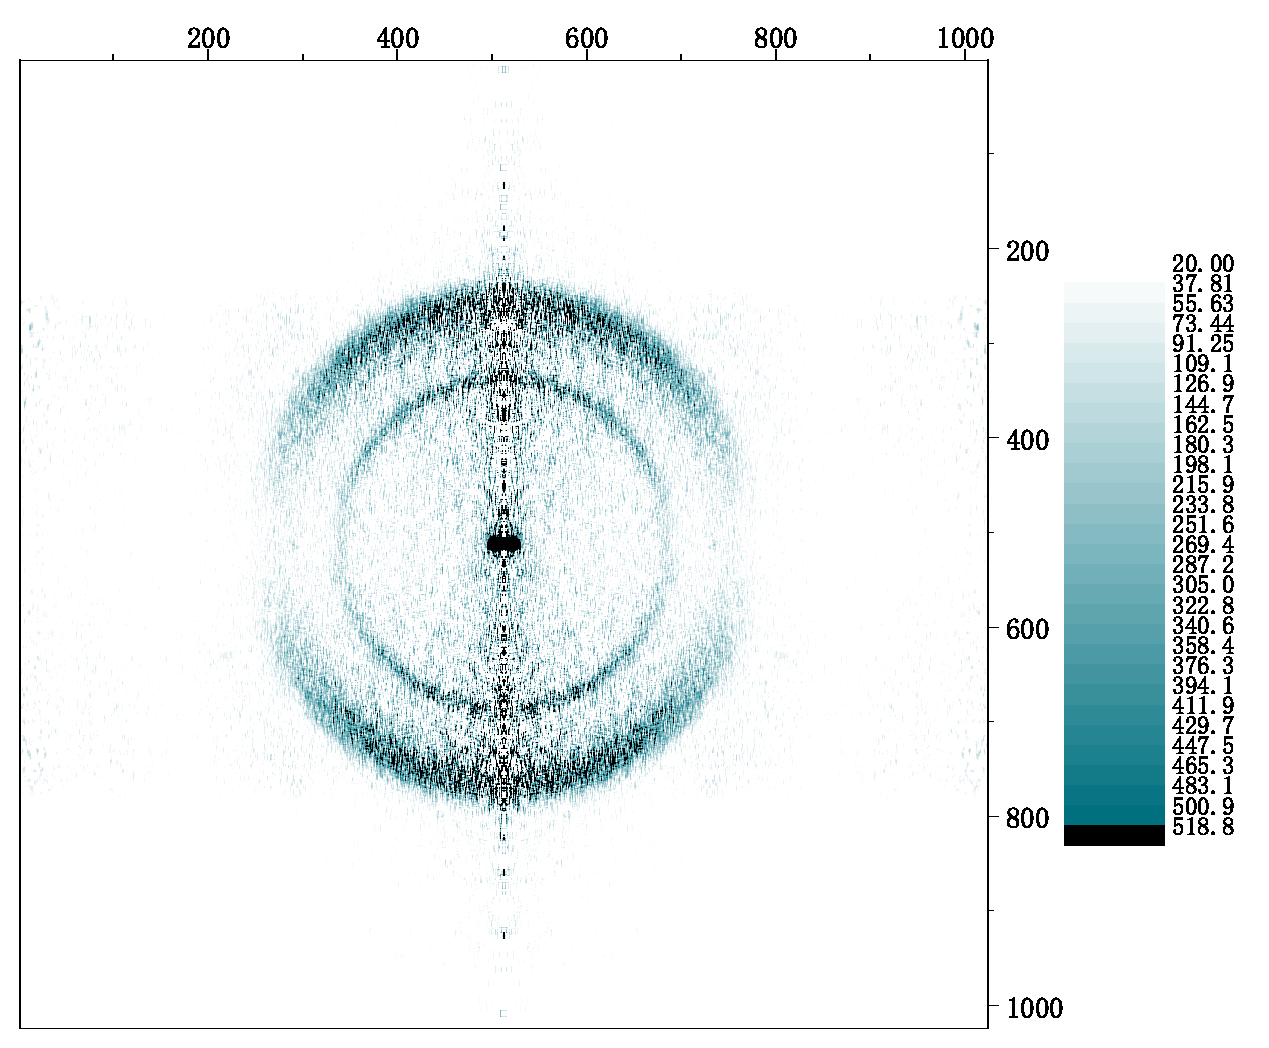
\includegraphics[width=4cm]{aring_463985.eps}};
			\node at (-2,-2){\includegraphics[width=4cm]{rdis_peak_463985.eps}};
			\node at (2,-2){\includegraphics[width=4cm]{adis_463985b.eps}};
			\node at (1.3,-3.2){\textcolor[RGB]{0,112,127}{\small $\beta \approx 1.23$}};
				\node at (-3.0,3.3){\textcolor[RGB]{0,112,127}{smear}};
			\node at (3.07,3.3){\textcolor[RGB]{0,112,127}{Abel${}^{-1}$}};
			}
\end{tikzpicture}
\end{figure}
\end{frame}
\begin{frame}{Peak 3}
\begin{figure}[H]
\centering
\begin{tikzpicture}
			\onslide<1,2>{\node at (0,0){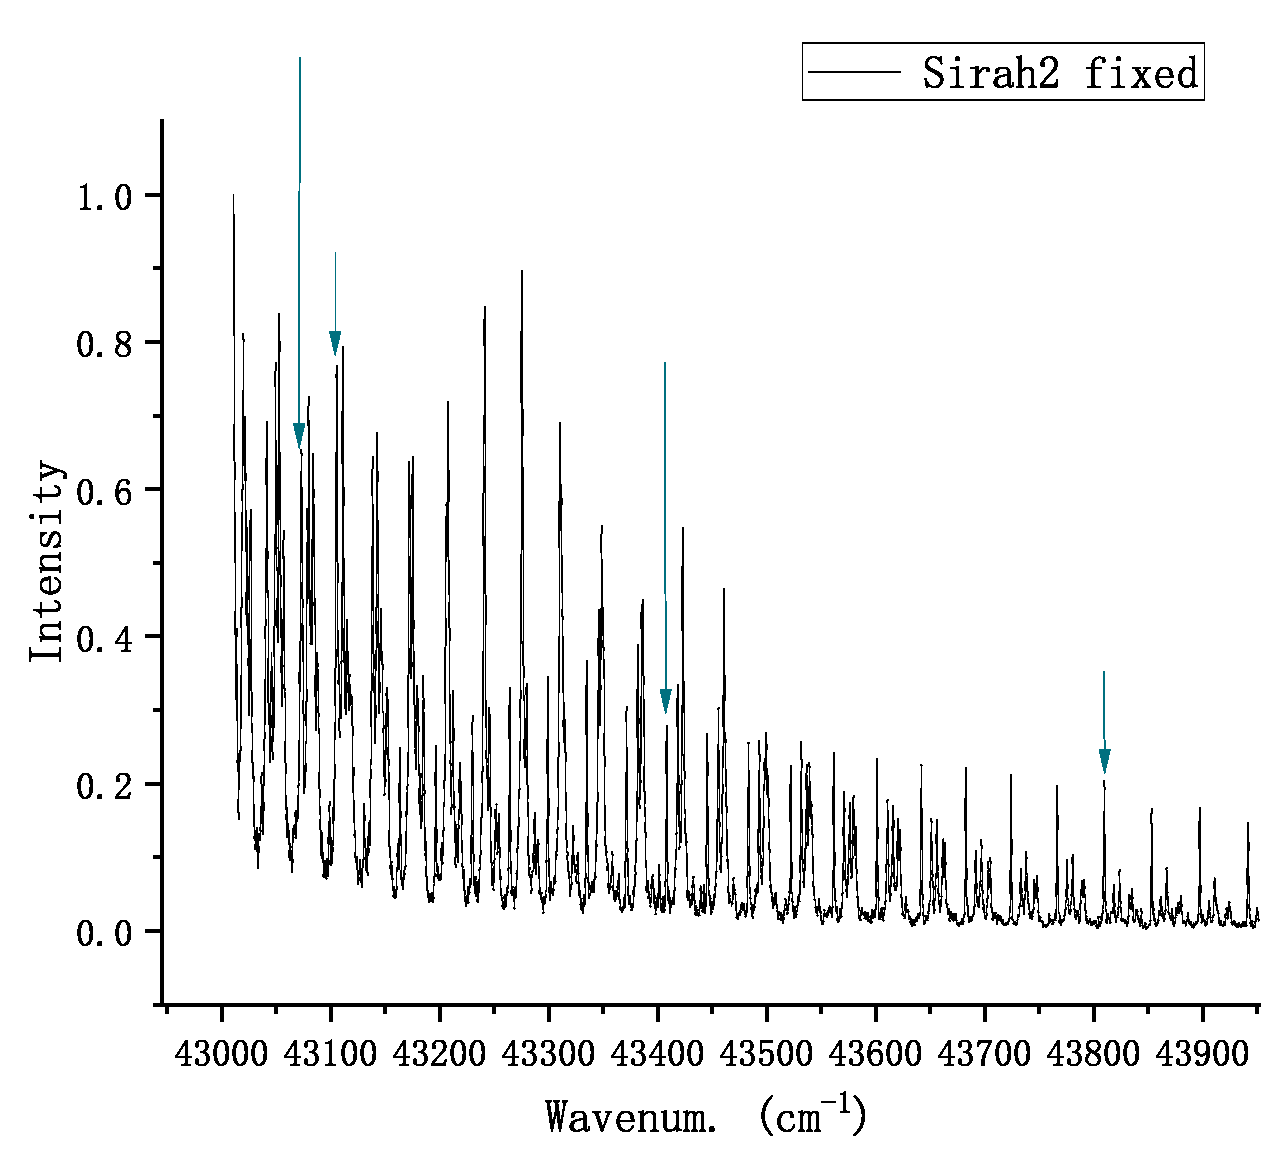
\includegraphics[width=0.6\textwidth]{scanmark.eps}};
			\filldraw[white] (-1.92,2.5) rectangle (-1.88,2.89);
			\node at (0.47,1.5){\textcolor[RGB]{0,112,127}{$\num{460.875}\unit{\nano \meter}$}};
			}
			\onslide<2>{
				\node at (2.03,2.4){{\quad\!}sR21(48.5)};
			}
			\onslide<3>{\node at (-1.55,2){\includegraphics[width = 4cm]{gring460745.eps}};
			\node at (2.45,2){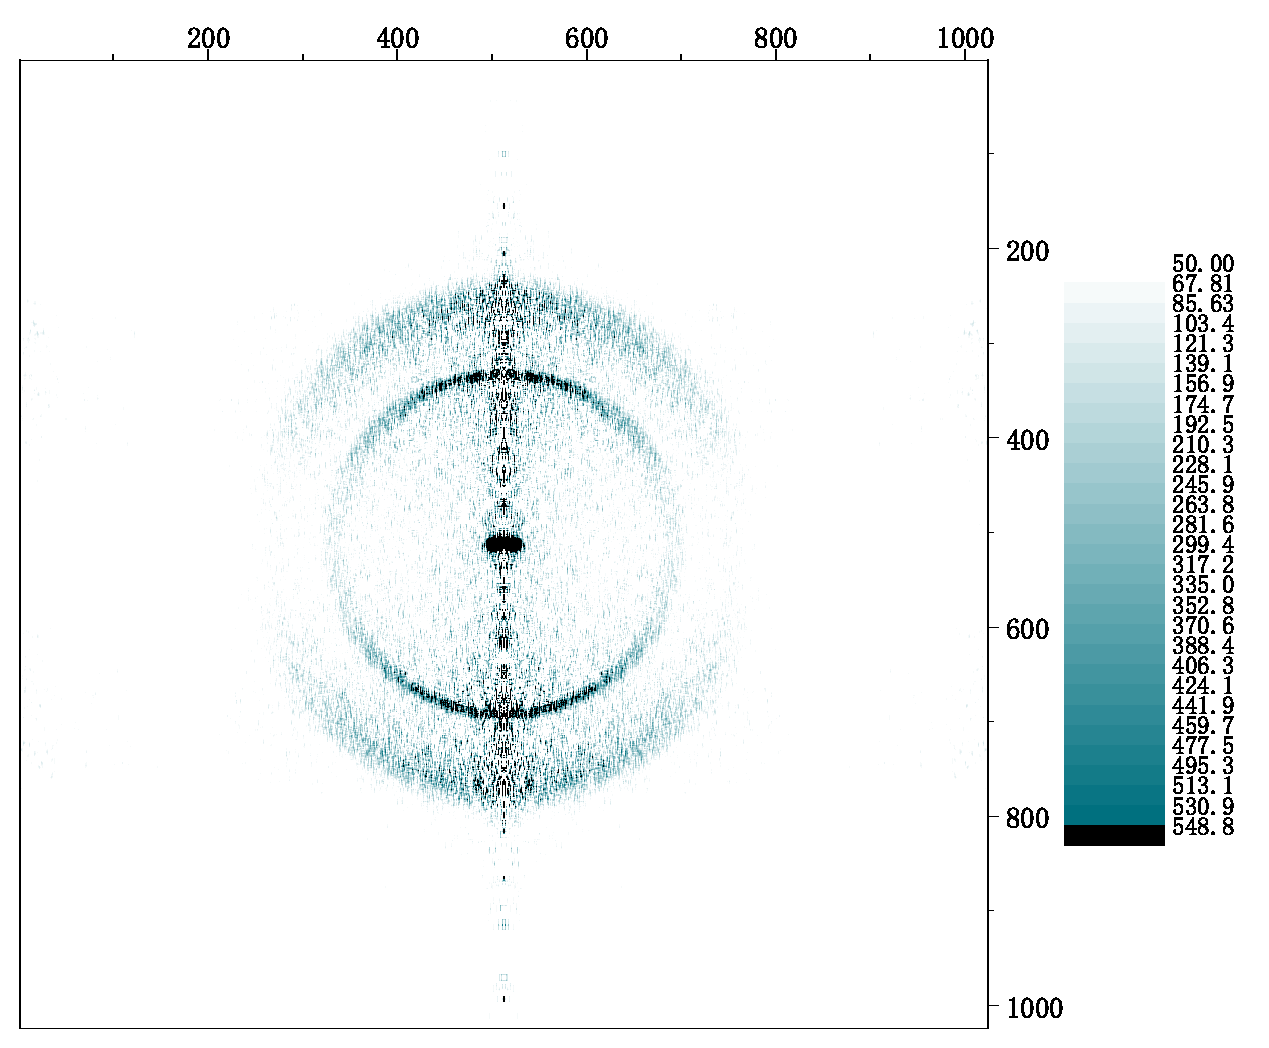
\includegraphics[width=4cm]{aring460745.eps}};
			\node at (-2,-2){\includegraphics[width=4cm]{rdis_peak_460745.eps}};
			\node at (2,-2){\includegraphics[width=4cm]{adis_460745b.eps}};
			\node at (1.3,-3.2){\textcolor[RGB]{0,112,127}{\small$\beta \approx 1.01$}};
				\node at (-3.0,3.3){\textcolor[RGB]{0,112,127}{smear}};
			\node at (3.07,3.3){\textcolor[RGB]{0,112,127}{Abel${}^{-1}$}};}
\end{tikzpicture}
\end{figure}
\end{frame}
\begin{frame}{Peak 4}
\begin{figure}[H]
\centering
\begin{tikzpicture}
		\onslide<1,2>{
			\node at (0,0){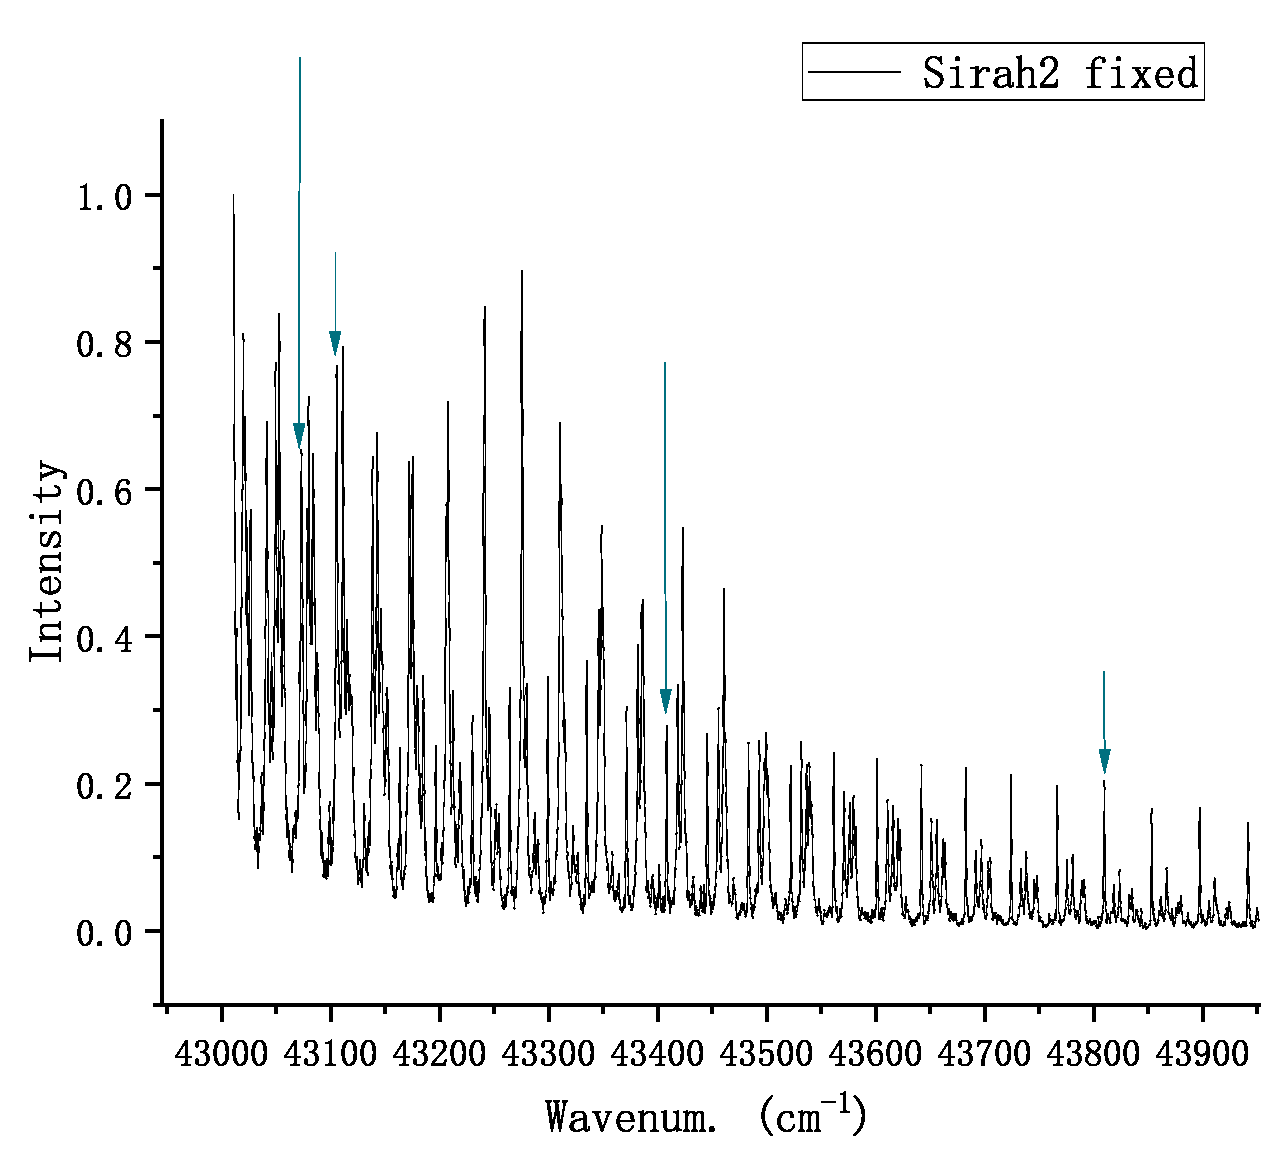
\includegraphics[width=0.6\textwidth]{scanmark.eps}};
			\filldraw[white] (-1.92,2.5) rectangle (-1.88,2.89);
			\node at (2.3,-0.25){\textcolor[RGB]{0,112,127}{$\num{456.659}\unit{\nano \meter}$}};
}
\onslide<2>{
			\node at (2.03,2.4){{\quad\!}sR21(58.5)};
			\node at (2.03,2){\textcolor{red}{{\quad\!}pQ12(76.5)}};
			\node at (2.03,1.6){\textcolor{red}{{\quad\!}pQ2(76.5)}};
}
			\onslide<3>{\node at (-1.55,2){\includegraphics[width = 4cm]{gring456528.eps}};
			\node at (2.45,2){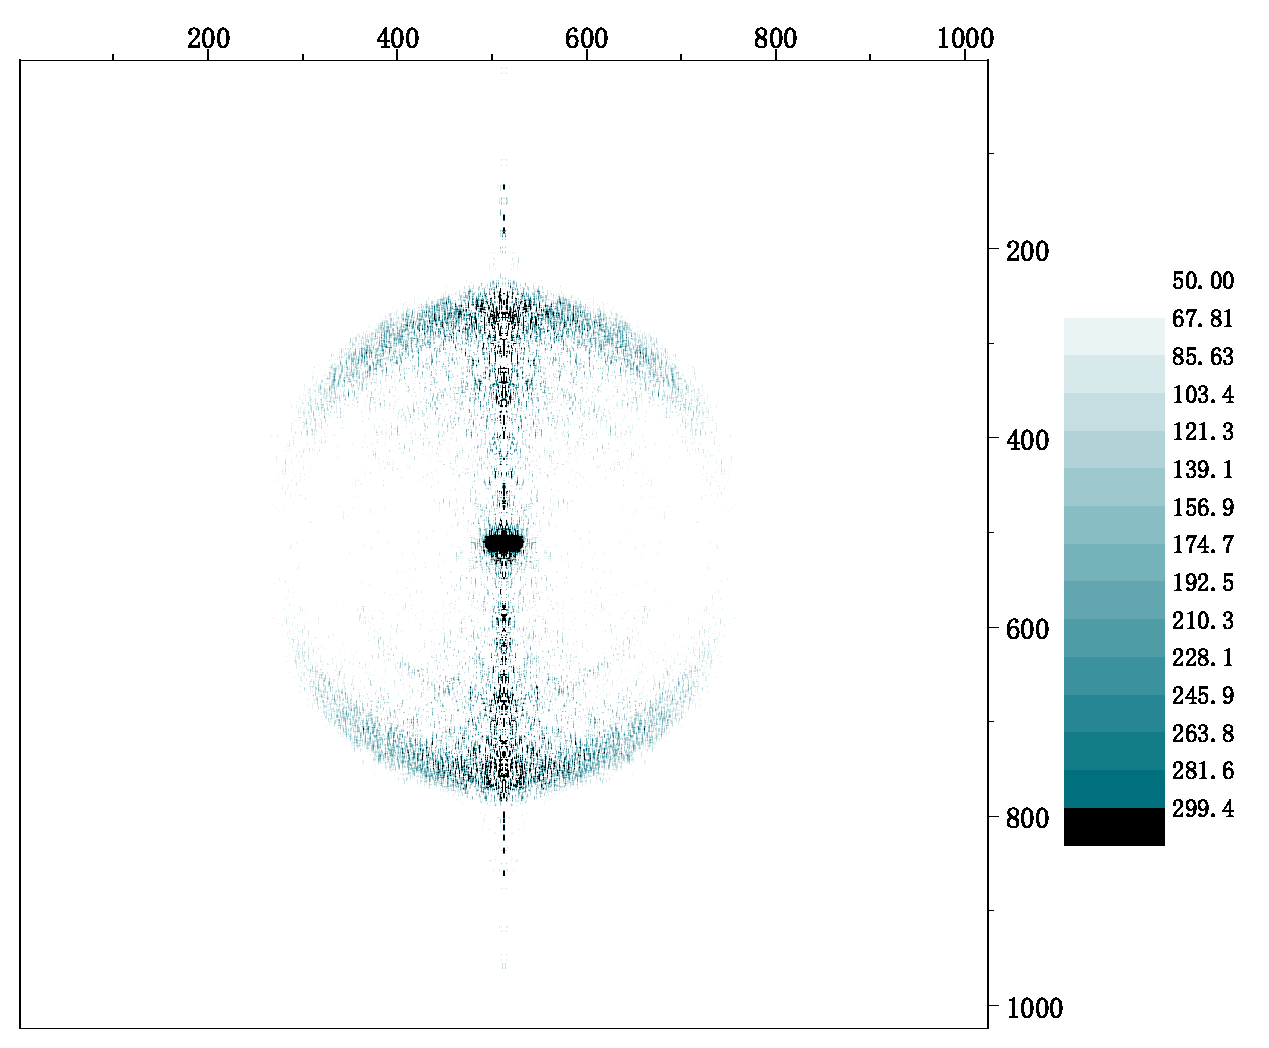
\includegraphics[width=4cm]{aring456528.eps}};
			\node at (-2,-2){\includegraphics[width=4cm]{rdis_peak_456528.eps}};
			\node at (2,-2){\includegraphics[width=4cm]{adis_456528b.eps}};
			\node at (1.3,-1.2){\small\textcolor[RGB]{0,112,127}{$\beta \approx 0.440$}};
				\node at (-3.0,3.3){\textcolor[RGB]{0,112,127}{smear}};
			\node at (3.07,3.3){\textcolor[RGB]{0,112,127}{Abel${}^{-1}$}};}
\end{tikzpicture}
\end{figure}
\end{frame}
\begin{frame}{Contents}
\tableofcontents[currentsection,currentsubsection]
\end{frame}
\subsection{Peak assignments}
\begin{frame}{\insertsubsection}
			\begin{table}
			\centering  	 
			\scriptsize
			\begin{tabularx}{0.9\textwidth}{llll}       
				$464.484 \unit{\nano \meter}$ &$464.114\unit{\nano \meter}$&$460.875 \unit{\nano \meter}$& $456.659 \unit{\nano \meter}$\\
				$\approx43058.49 \unit{\per \centi \meter}$ &   $\approx43092.81\unit{\per \centi \meter}$ &  $\approx 43395.69\unit{\per \centi \meter}$ & $\approx 43796.34\unit{\per \centi \meter} $\\
				\toprule   
				$\text{px}=258$ & $\text{px}=258$ & $\text{px}=258$ &$ \text{px}=249$ \\  
				\midrule 
				$rR2\:44.5$ & $rR2\:45.5$ &  &$sR21\:58.5$\\  
				\textcolor[RGB]{0,112,127}{$qR12\:51.5$} & \textcolor[RGB]{0,112,127}{$qR12 \:51.5$} &  $sR21\:48.5$ & \textcolor[RGB]{0,112,127}{$pQ12 \:76.5$} \\ 
				\textcolor[RGB]{0,112,127}{$qQ2\: 51.5$} & \textcolor[RGB]{0,112,127}{$qQ2\: 51.5$} &   & \textcolor[RGB]{0,112,127}{$pP2\: 76.5$} \\ 
				\bottomrule    
			\end{tabularx}%  
			\label{tab:addlabel}%
		\end{table}%
		\begin{alertblock}{Notice}
			\textcolor[RGB]{0,112,127}{Colored} assignments are mismatched, and will not be used to calculate.
		\end{alertblock}
	\end{frame}
	\begin{frame}{Contents}
		\tableofcontents[currentsection,currentsubsection]
	\end{frame}
	\subsection{Speed correction}
	\subsubsection{Trans. energy of \ce{NO}}
	\begin{frame}{\insertsubsection}{\insertsubsubsection}
		\begin{table}[htbp]
			\centering
			\tiny
			\begin{tabularx}{0.9\textwidth}{lccc}
				& $E_\text{total}$ & $E_\text{bond}(\ce{O-NO})$ \footfullcite{ono}& $E_\text{int.}(\ce{NO})$ \\
				\toprule
				Peak 1 & \multirow{2}[2]{*}{$\num{43058.49}\unit{\per \centi \meter}$} & \multirow{8}[8]{*}{$\num{25128.57}\unit{\per \centi \meter}$} & \multirow{2}[2]{*}{\qquad\quad\,\;\;$E (v = 1)+ E( J = 44 )$\qquad\quad\,\;\;} \\
				$\num{464.484}\unit{\nano\meter}$ & & & \\
				\cmidrule{1-2}\cmidrule{4-4}
				Peak 2 & \multirow{2}[2]{*}{$\num{43092.81}\unit{\per \centi \meter}$} & & \multirow{2}[2]{*}{\qquad\quad\,\;\;$E (v = 1)+ E( J = 45 )$\qquad\quad\,\;\;} \\
				$\num{464.114}\unit{\nano\meter}$ & & & \\
				\cmidrule{1-2}\cmidrule{4-4}
				Peak 3 & \multirow{2}[2]{*}{$\num{43395.69}\unit{\per \centi \meter}$} & & \multirow{2}[2]{*}{\qquad\quad\,\;\;$E (v = 1)+ E( J = 48 )$\qquad\quad\,\;\;} \\
				$\num{460.875}\unit{\nano\meter}$ & & & \\
				\cmidrule{1-2}\cmidrule{4-4}
				Peak 4 & \multirow{2}[2]{*}{$\num{43796.34}\unit{\per \centi \meter}$} & & \multirow{2}[2]{*}{\qquad\quad\,\;\;$E (v = 1)+ E( J = 58 )$\qquad\quad\,\;\;} \\
				$\num{456.659}\unit{\nano\meter}$ & & & \\
				\bottomrule
			\end{tabularx}
		\end{table}
	\end{frame}
	\begin{frame}{\insertsubsection}{\insertsubsubsection}
		\begin{table}[htbp]
			\centering
			\tiny
			\begin{tabularx}{0.9\textwidth}{lccc}
				& $E_\text{total}$ & $E_\text{bond}(\ce{O-NO})$\footfullcite{ono} & $E_\text{int.}(\ce{NO})$ \\
				\toprule
				Peak 1 & \multirow{2}[2]{*}{$\num{43058.49}\unit{\per \centi \meter}$} & \multirow{8}[8]{*}{$\num{25128.57}\unit{\per \centi \meter}$} & \multirow{2}[2]{*}{$\num{3525.0743625}\unit{\per \centi \meter}+ E( J = 44 )$} \\
				$\num{464.484}\unit{\nano\meter}$ & & & \\
				\cmidrule{1-2}\cmidrule{4-4}
				Peak 2 & \multirow{2}[2]{*}{$\num{43092.81}\unit{\per \centi \meter}$} & & \multirow{2}[2]{*}{$\num{3525.0743625}\unit{\per \centi \meter}+ E( J = 45 )$} \\
				$\num{464.114}\unit{\nano\meter}$ & & & \\
				\cmidrule{1-2}\cmidrule{4-4}
				Peak 3 & \multirow{2}[2]{*}{$\num{43395.69}\unit{\per \centi \meter}$} & & \multirow{2}[2]{*}{$\num{3525.0743625}\unit{\per \centi \meter}+ E( J = 48 )$} \\
				$\num{460.875}\unit{\nano\meter}$ & & & \\
				\cmidrule{1-2}\cmidrule{4-4}
				Peak 4 & \multirow{2}[2]{*}{$\num{43796.34}\unit{\per \centi \meter}$} & & \multirow{2}[2]{*}{$\num{3525.0743625}\unit{\per \centi \meter}+ E( J = 58 )$} \\
				$\num{456.659}\unit{\nano\meter}$ & & & \\
				\bottomrule
			\end{tabularx}
		\end{table}
		\onslide<2>{\begin{block}{Vib. energy level\footfullcite{vj}}
			$E\left( v\right)  = \omega_e\left( v+\frac{1}{2} \right) -\omega_e x_e\left( v+\frac{1}{2} \right)^2+\omega_e y_e\left( v+\frac{1}{2} \right)^3$.
		\end{block}}
	\end{frame}	
	\begin{frame}{\insertsubsection}{\insertsubsubsection}
		\begin{table}[htbp]
			\centering
			\tiny
			\begin{tabularx}{0.9\textwidth}{lccc}				
				& $E_\text{total}$ & $E_\text{bond}(\ce{O-NO})$ \footfullcite{ono}& $E_\text{int.}(\ce{NO})$ \\
				\toprule
				Peak 1 & \multirow{2}[2]{*}{$\num{43058.49}\unit{\per \centi \meter}$} & \multirow{8}[8]{*}{$\num{25128.57}\unit{\per \centi \meter}$} & \multirow{2}[2]{*}{\qquad\qquad\,\;\;$\num{6848.563763}\unit{\per \centi \meter}$\qquad\qquad\,\;\;} \\
				$\num{464.484}\unit{\nano\meter}$ & & & \\
				\cmidrule{1-2}\cmidrule{4-4}
				Peak 2 & \multirow{2}[2]{*}{$\num{43092.81}\unit{\per \centi \meter}$} & & \multirow{2}[2]{*}{$\num{6999.631462}\unit{\per \centi \meter}$} \\
				$\num{464.114}\unit{\nano\meter}$ & & & \\
				\cmidrule{1-2}\cmidrule{4-4}
				Peak 3 & \multirow{2}[2]{*}{$\num{43395.69}\unit{\per \centi \meter}$} & & \multirow{2}[2]{*}{$\num{7472.976923}\unit{\per \centi \meter}$} \\
				$\num{460.875}\unit{\nano\meter}$ & & & \\
				\cmidrule{1-2}\cmidrule{4-4}
				Peak 4 & \multirow{2}[2]{*}{$\num{43796.34}\unit{\per \centi \meter}$} & & \multirow{2}[2]{*}{$\num{9269.004023}\unit{\per \centi \meter}$} \\
				$\num{456.659}\unit{\nano\meter}$ & & & \\
				\bottomrule
			\end{tabularx}
		\end{table}
		\onslide<2>{\begin{block}{Rot. energy level\footfullcite{vj}}
			$E\left( J\right) = B_v \left( J^2 + J\right) $
		\end{block}}
	\end{frame}
%	$E_\text{trans} $ $= E_\text{total} -E_\text{bond}(\ce{O-NO})-E_\text{int.}(\ce{O})- E_\text{int.}(\ce{O}) $
	\begin{frame}{\insertsubsection}{\insertsubsubsection}
\begin{table}[htbp]
	\centering
	\tiny
	\begin{tabularx}{0.9\textwidth}{l|cc}
		\multicolumn{1}{l}{\multirow{2}[1]{*}{$E_\text{int.}(\ce{O})$}} & \multicolumn{1}{l}{$E_\text{trans} (total)\approx2.88 E_\text{trans}(\ce{NO}) $} & \multicolumn{1}{l}{$E_\text{trans}(\ce{NO})$} \\
		\multicolumn{1}{l}{} & \multicolumn{1}{l}{$= E_\text{total} -E_\text{bond}(\ce{O-NO})-E_\text{int.}(\ce{O})- E_\text{int.}(\ce{O}) $} & \multicolumn{1}{l}{ $= \frac{1}{2}m(\ce{NO})v^2(\ce{NO})$} \\
		\midrule
		\multirow{2}[1]{*}{$^3 P_2$} & $11081.356237\unit{\per \centi\meter}$ & $1923.84656892361\unit{\per \centi\meter}$ \\
		& $10964.608538\unit{\per \centi\meter}$ & $1903.57787118055\unit{\per \centi\meter}$ \\
		\multirow{2}[1]{*}{($\num{0}\unit{\per \centi \meter}$)} & $10794.143077\unit{\per \centi\meter}$ & $1873.98317309028\unit{\per \centi\meter}$ \\
		& $9398.765977\unit{\per \centi\meter}$ & $1631.73020434028\unit{\per \centi\meter}$ \\
		\midrule
		\multirow{2}[1]{*}{$^3 P_1$} & $10922.731237\unit{\per \centi\meter}$ & $1896.30750642361\unit{\per \centi\meter}$ \\
		& $10805.983538\unit{\per \centi\meter}$ & $1876.03880868055\unit{\per \centi\meter}$ \\
		\multirow{2}[1]{*}{($\num{158.625}\unit{\per \centi \meter}$)} & $10635.518077\unit{\per \centi\meter}$ & $1846.44411059028\unit{\per \centi\meter}$ \\
		& $9240.140977\unit{\per \centi\meter}$ & $1604.19114184028\unit{\per \centi\meter}$ \\
		\midrule
		\multirow{2}[1]{*}{$^3 P_0$} & $10854.379237\unit{\per \centi\meter}$ & $1884.44083975695\unit{\per \centi\meter}$ \\
		& $10737.631538\unit{\per \centi\meter}$ & $1864.17214201389\unit{\per \centi\meter}$ \\
		\multirow{2}[1]{*}{($\num{226.977}\unit{\per \centi \meter}$)} & $10567.166077\unit{\per \centi\meter}$ & $1834.57744392361\unit{\per \centi\meter}$ \\
		& $9171.788977\unit{\per \centi\meter}$ & $1592.32447517361\unit{\per \centi\meter}$ \\
		\bottomrule
	\end{tabularx}%
\end{table}%
\end{frame}
	\begin{frame}{\insertsubsection}{\insertsubsubsection}
	% Table generated by Excel2LaTeX from sheet 'Sheet1'
\begin{table}[htbp]
	\centering
	\tiny
	\begin{tabular}{l|cc}
		\multicolumn{1}{l}{\multirow{2}[1]{*}{$E_\text{int.}(\ce{O})$}} & \multicolumn{1}{l}{$v(\ce{NO}) $} & \multirow{2}[1]{*}{$\Delta y $} \\
		\multicolumn{1}{l}{} & \multicolumn{1}{l}{$= \sqrt { \frac{2E_\text{trans}(\ce{NO})}{m(\ce{NO})} }$} &  \\
		\midrule
		\multirow{2}[1]{*}{$^3 P_2$} & $1486.240384\unit{\meter \per \second}$ & 258 px \\
		& $1478.3905065\unit{\meter \per \second}$ & 258 px \\
		\multirow{2}[1]{*}{($\num{0}\unit{\per \centi \meter}$)} & $1466.8533085\unit{\meter \per \second}$ & 258 px \\
		& $1368.7622455\unit{\meter \per \second}$ & 249 px \\
		\midrule
		\multirow{2}[1]{*}{$^3 P_1$} & $1475.5645855\unit{\meter \per \second}$ & 258 px \\
		& $1467.6576085\unit{\meter \per \second}$ & 258 px \\
		\multirow{2}[1]{*}{($\num{158.625}\unit{\per \centi \meter}$)} & $1456.0353685\unit{\meter \per \second}$ & 258 px \\
		& $1357.162647\unit{\meter \per \second}$ & 249 px \\
		\midrule
		\multirow{2}[1]{*}{$^3 P_0$} & $1470.940464\unit{\meter \per \second}$ & 258 px \\
		& $1463.0084955\unit{\meter \per \second}$ & 258 px \\
		\multirow{2}[1]{*}{($\num{226.977}\unit{\per \centi \meter}$)} & $1451.3490265\unit{\meter \per \second}$ & 258 px \\
		& $1352.133667\unit{\meter \per \second}$ & 249 px \\
		\bottomrule
	\end{tabular}%
\end{table}%
\end{frame}

%	
%	
%\begin{frame}
%	\begin{columns}
	%		\begin{column}{0.65\textwidth}
		%	
		%		\end{column}
	%		\vrule
	%		\begin{column}{0.35\textwidth}
		%			
		%		\end{column}
	%	\end{columns}
%\end{frame}
%	
%	
%	
%	
%
%	\begin{frame}
%		このスライドはソースコードが\qrcode[hyperlink,height=2cm]{https://github.com/xiaoyuleiba/Machinetime-Report}にて公開される。
%	\end{frame}
\section*{Reference}
\begin{frame}{\insertsection}
	\printbibliography
\end{frame}
\end{document}









